%  section on run scenarios

% CHAPTER ON ILC RUNNING SCENARIOS

Amoung the advantages of $e^+e^-$ colliders is the ability to collect datasets with different center-of-mass energies and beam polarisation settings, according to the neeeds of the various physics measurements.
While each measurement has its prefered data-taking mode, the combination with datasets collected other beam energies and/or beam polarisations provide important robustness against systematic uncertainties.

Any physics projection will depend on the exact assumptions on the assumed running scenario, i.e.\ the integrated luminosity collected at each considered center-of-mass energy with each polarisation setting.


The interplay of different datasets has been studied in detail in~\cite{Barklow:2015tja}, with a special focus on optimising the Higgs precision measurements. 

{\color{red} HERE: Tables with integrated luminsoities and polarisation mit from~\cite{Barklow:2015tja}}

{\color{red} Time dependence: explain why need longer when starting at 250\,\GeV}

{\color{red} explain new beam parameters, cite machine staging report}


%%%%%%%%%%%%%%%%%%%%%%%%%%%%%%%%%%%%%%%%%%%%%%%%%%%%%%%%%%%%%%%%%%%%%%%%%
\begin{figure}
\begin{center}
\includegraphics[width=0.75\hsize]{chapters/figures/lumi_H-20.pdf}
\end{center}
\caption{The nominal 20-year running program for the 500-GeV-ILC~\cite{Barklow:2015tja}.}
\label{fig:H20}
\end{figure}
%%%%%%%%%%%%%%%%%%%%%%%%%%%%%%%%%%%%%%%%%%%%%%%%%%%%%%%%%%%%%%%%%%%%%%%%%%%

%%%%%%%%%%%%%%%%%%%%%%%%%%%%%%%%%%%%%%%%%%%%%%%%%%%%%%%%%%%%%%%%%%%%%%%%%
\begin{figure}
\begin{center}
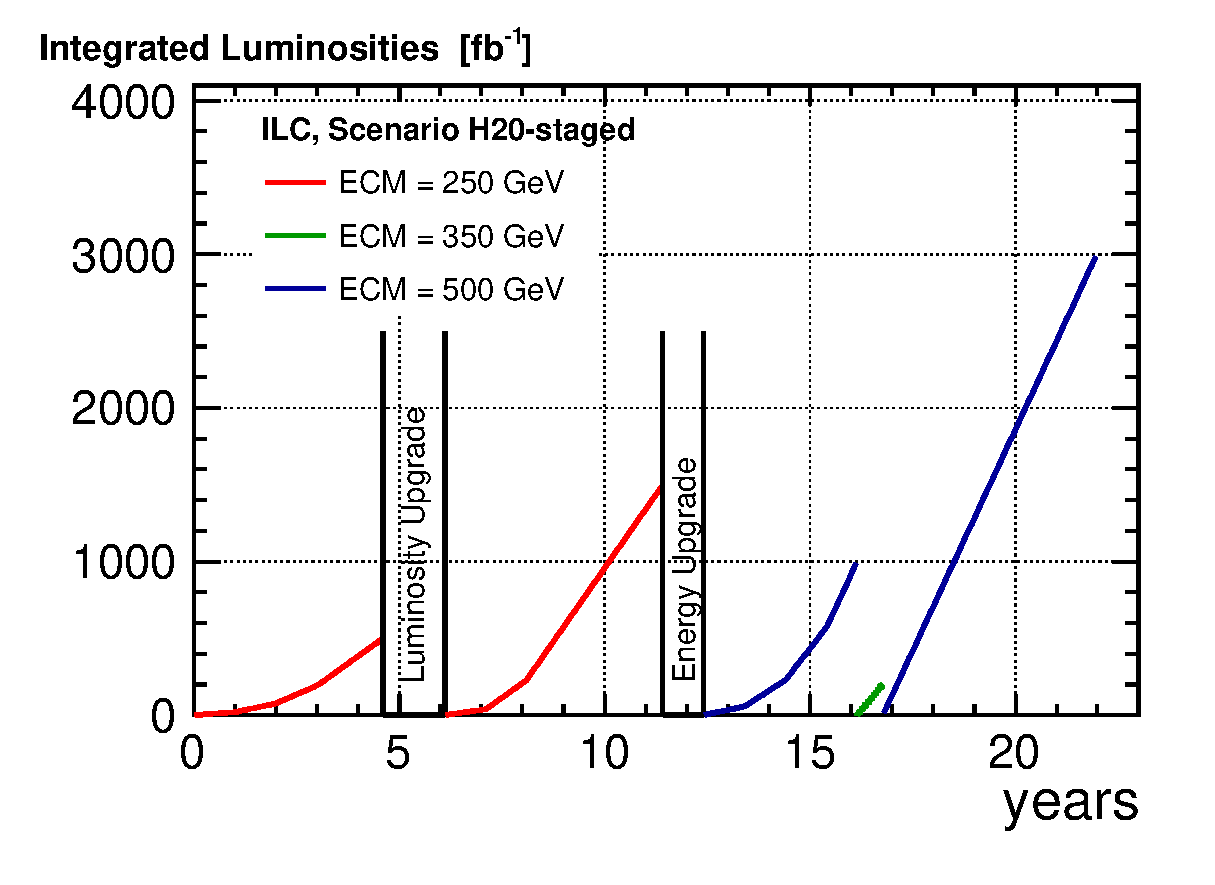
\includegraphics[width=0.75\hsize]{chapters/figures/lumi_H20-staged}
\end{center}
\caption{The nominal 22-year running program for the staged ILC, starting operation at 250\,\GeV ~\cite{ILC250}. The integrated luminosities are the same of for the original H20 scenario.}
\label{fig:H20staged}
\end{figure}
%%%%%%%%%%%%%%%%%%%%%%%%%%%%%%%%%%%%%%%%%%%%%%%%%%%%%%%%%%%%%%%%%%%%%%%%%%%
